\documentclass[11pt]{beamer} % mathserif for normal math fonts.
\usefonttheme[onlymath]{serif}
\usepackage[utf8]{inputenc}
\usepackage[swedish,english]{babel}
\usepackage{microtype}
\usepackage{calc}
\usepackage{amsmath,mathtools}
\usepackage[backend=biber]{biblatex}
\usepackage{contmech}
%\usepackage{subfig}
%\usepackage{siunitx}
%\usepackage{movie15}
\usepackage{wasysym}
\usepackage{multimedia}
\usepackage{grffile}
\usepackage{tikz}
\usepackage{pgfplots}

%\pgfplotsset{compat=newest}
\pgfplotsset{compat=1.6}
\usetikzlibrary{shapes,arrows}

\newcommand{\highlight}[1]{{\color{red}#1}}
\newcommand{\downlight}[1]{{\color{gray}#1}}
\DeclarePairedDelimiter{\homgen}{\langle}{\rangle_\rve}
\DeclarePairedDelimiter{\shomgen}{\langle\!\langle}{\rangle\!\rangle_\rve}
\DeclarePairedDelimiter{\jmp}{[\![}{]\!]}
\newcommand{\jump}[1]{[\![#1]\!]}
\newcommand{\prescribed}{\mathrm{pre}}
\newcommand{\on}{\quad\text{ on }}
\renewcommand{\dev}{\mathrm{d}}
\renewcommand{\vol}{\mathrm{v}}
\newcommand{\per}{\mathrm{per}}
\newcommand{\volume}{|\Omega_\rve|}
\newcommand{\ded}{\mathrm{d}}
\newcommand{\dep}{\mathrm{p}}
\newcommand{\Periodic}{\mathrm{P}}
\newcommand{\external}{\mathrm{ext}}
\newcommand{\surf}{\mathrm{s}}
\newcommand{\pore}{\mathrm{pore}}
\newcommand{\particle}{\mathrm{part}}
\newcommand{\devop}{\ts\epsilon_\dev}
\newcommand{\densinv}{\eta}
\newcommand{\dens}{\eta^{-1}}
\newcommand{\epspargs}{\{{\bar{\ts d}}_\dev, \bar{p}\}}
\newcommand{\rve}{
  {\mathchoice
   {\mbox{\scalebox{0.67}{$\Box$}}}
   {\mbox{\scalebox{0.67}{$\Box$}}}
   {\mbox{\scalebox{0.5}{$\Box$}}}
   {\mbox{\scalebox{0.375}{$\Box$}}}
  }
}
%\usepgfplotslibrary{patchplots}
%\usepgfplotslibrary{groupplots}
%\pgfplotsset{compat=1.3}

\newcommand{\roughcite}[1]{\textsc{#1}}
\renewcommand{\alert}[1]{\textbf{#1}}

\setbeamersize{text margin left=.3cm,text margin right=.3cm}

\usetheme[titleflower=true]{chalmers}
\title{
On computational modeling of sintering based on homogenization
}
\author[Mikael \"Ohman WCCM-ECCM  --- 2014-07-22]{Mikael \"Ohman\\Kenneth Runesson\\Fredrik Larsson}
\institute{Department of Applied Mechanics\\ Chalmers University of Technology\\
mikael.ohman@chalmers.se
}
%\titlepageextra{2012}% session: Multiple-scale physics and computation
\date{2014-07-22}
%\footer{\insertshortauthor\ 2\textsuperscript{nd} ICMM}
\titlepagelogofile{Avancez_gold}

% Bibliography
%\bibliography{references_extended}

% Speeds up compilation.
% \usetikzlibrary{external}
% \tikzexternalize


\addbibresource{Multiscale.bib} % New command, use if available
\addbibresource{Sintering.bib}

\begin{document}

\section{Title page}
\begin{frame}[plain]
 \titlepage
\end{frame}

%\section{Acknowledgement}
%\begin{frame}
% \frametitle{Acknowledgement}
% \begin{center}
% Funding:
% \\
% Swedish Research Council (Vetenskapsrådet)
% \\
% Chalmers University of Technology
% \\[2em]
% Supervisors:\\
% Professor Kenneth Runesson \\
% Professor Fredrik Larsson
% \end{center}
%\end{frame}

\section{Outline}
\begin{frame}
 \frametitle{Outline}

\begin{itemize}
 \item Mixed formulation for incompressible elasticity
 \item Problem with traditional boundary conditions
 \item Derived macroscale problem
 \item Weakly periodic boundary condition
 \item Conclusions
\end{itemize}
\end{frame}

%%%%%%%%%%%%%%%%%%%%%%%%%%%%%%%%%%%%%%%%%%%%%%%%%%%%%%%%%%%%%%%%%%%%%%%%%%%%%%%%%%%%%%%%%%%%%%%%%%%
\section{Theory}

%%%%%%%%%%%%%%%%%%%%%%%%%%%%%%%%%%%%%%%%%%%%%%%%%%%%%%%%%%%%%%%%%%%%%%%%%%%%%%%%%%%%%%%%%%%%%%%%%%%
\begin{frame}
 \frametitle{Fine-scale problem}
 \begin{itemize}
  \item Mixed displacement-pressure formulation
  \begin{align*}
   -[\hat{\ts\sigma}_\dev(\ts\epsilon_\dev) - p\ts I]\cdot\ta\nabla &= \ta 0 \text{ in } \Omega
    \\
    \hat{e}(p) - \ta u\cdot\ta\nabla &= 0\text{ in } \Omega%, \quad \Omega = \cup_\alpha \Omega_\alpha
  \end{align*}
  \item Example material model, isotropic linear elasticity
  \begin{gather*}
   \hat{\ts\sigma}_\dev(\ts\epsilon_\dev) \defeq 2 G \ts\epsilon_\dev\\
   \hat{\ts\sigma}_\dev(\ts\epsilon_\dev) = \ts\sigma + p\ts I,\quad \ts\epsilon_\dev \defeq [\ta u\outerp \diff]_\dev^\sym
   \\
   \hat{e}(p) \defeq -C\,p
  \end{gather*}
  \item For compressible cases, the bulk modulus is $ K = C^{-1}$
  \item Subscript $\dev$ denotes deviatoric tensor: $\bullet_\dev = \bullet - \frac13 [\bullet:\ts I]\ts I$
 \end{itemize}
\end{frame}

%%%%%%%%%%%%%%%%%%%%%%%%%%%%%%%%%%%%%%%%%%%%%%%%%%%%%%%%%%%%%%%%%%%%%%%%%%%%%%%%%%%%%%%%%%%%%%%%%%%
\begin{frame}
 \frametitle{Weak form of ``fine-scale'' problem}
 \begin{itemize}
  \item %Sintering particles occupying domain $\Omega$ with internal pore boundary $\Gamma^\pore$:
Find $(\ta u,p)\in \set U \times \set P$ such that
\begin{align*}
  \int_{\mathrlap{\Omega}} \;[\hat{\ts\sigma}_\dev([\ta u\outerp\diff]_\dev^\sym)-p\ts I]\dprod[\delta\ta u\outerp\ta\nabla]\dif v &=
   0 %\int_{\mathrlap{\Gamma^\pore}} \;\gamma_\surf[\delta\ta u\cdot\hat{\ta\nabla}] \dif a
    % +\int_{\mathrlap{\Gamma_\Neumann^\external}} \;\ta t_p\cdot\delta\ta u\dif a \; 
    && \forall \delta \ta u\in \set U^0
\\
  \int_{\mathrlap{\Omega}} \;[\hat{e}(p) - \ta u\cdot\ta\nabla]\delta p \dif v &= 0 && \forall \delta p\in \set P
\end{align*}
 \end{itemize}
\end{frame}


%%%%%%%%%%%%%%%%%%%%%%%%%%%%%%%%%%%%%%%%%%%%%%%%%%%%%%%%%%%%%%%%%%%%%%%%%%%%%%%%%%%%%%%%%%%%%%%%%%%
\begin{frame}
 \frametitle{Problem with classical boundary conditions}
  \begin{itemize}
   \item As $C\to 0$, the volumetric part of the macroscopic strain can no longer be controlled in an RVE. Classical (Dirichlet and Neumann) boundary conditions for homogenization breaks down.
   \item Solution presented:
    \begin{center}
    %\fullcite{ohman_variationally_2014}
     Mikael Öhman, Kenneth Runesson, and Fredrik Larsson.
     \\%[1em]
    \textit{On the variationally consistent computational homogenization of elasticity in the incompressible limit}.
     \\%[1em]
     Advanced Modeling and Simulation in Engineering Sciences (2014). Under review
    \end{center}
  \end{itemize}
\end{frame}

%%%%%%%%%%%%%%%%%%%%%%%%%%%%%%%%%%%%%%%%%%%%%%%%%%%%%%%%%%%%%%%%%%%%%%%%%%%%%%%%%%%%%%%%%%%%%%%%%%%
\begin{frame}
 \frametitle{Variationally Consistent Homogenization (VCH)}
\begin{itemize}
 \item Volume average operators over the RVE-window $\Omega_\rve$
\begin{align*}
 \homgen{\bullet} \defeq \frac{1}{\volume} \int_{\Omega_\rve} \bullet \dif V%,\quad \Omega_\rve^\particle \defeq \Omega_\rve \cap \Omega^\particle
% \\
%  \shomgen{\bullet} \defeq \frac{1}{\volume} \int_{\Gamma^\pore_\rve} \bullet \dif S%,\quad \Gamma^\pore_\rve \defeq \Omega_\rve \cap \Gamma^\pore
\end{align*}
 \item Decompose the fields into macroscopic and fluctuating parts:
 \begin{align*}
  \ta u = \ta u^\macro + \ta u^\fluct
   \\
  p = p^\macro + p^\fluct
 \end{align*}
 \item Variationally Consistent Homogenization $\leadsto$ macroscale problem
\end{itemize}
\end{frame}

%%%%%%%%%%%%%%%%%%%%%%%%%%%%%%%%%%%%%%%%%%%%%%%%%%%%%%%%%%%%%%%%%%%%%%%%%%%%%%%%%%%%%%%%%%%%%%%%%%%
\begin{frame}
 \frametitle{Variationally Consistent Macrohomogenity Condition}
\begin{itemize}
 \item Variationally Consistent Macrohomogeneity condition (VCMC):
 \begin{center}
  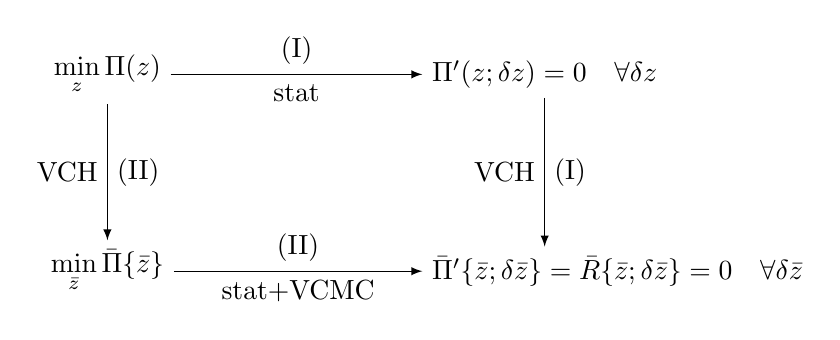
\begin{tikzpicture}
 \newcommand{\ub}{z}
 \node (A) at(0,0) {$\displaystyle\min_{\ub} \Pi(\ub)$};
 \node (B) at(0,-2.5) {$\displaystyle\min_{\bar{\ub}} \bar{\Pi}\{\bar{\ub}\}$};

 \node[right] (C) at(4,0) {$\Pi'(\ub;\delta\ub) = 0 \quad\forall \delta\ub$};
 \node[right] (D) at(4,-2.5) {$\bar{\Pi}'\{\bar\ub;\delta\bar\ub\} = \bar{R}\{\bar\ub;\delta\bar\ub\} = 0 \quad\forall \delta\bar\ub$};

% \node at(5,-3.5) {$=\bar{R}\{\ub;\delta\ub\}$};

 \draw[-latex] (A) -- coordinate(AB) (B);
 \draw[-latex] (B) -- coordinate(BD) (D);

 \draw[-latex] (A) -- coordinate(AC) (C);
 \draw[-latex] (C) -- coordinate(CD) (C |- D.north);

 \node[left] at (AB) {VCH};
 \node[right] at (AB) {(II)};

 \node[below] at (BD) {stat+VCMC};
 \node[above] at (BD) {(II)};


 \node[below] at (AC) {stat};
 \node[above] at (AC) {(I)};

 \node[left] at (CD) {VCH};
 \node[right] at (CD) {(I)};


\end{tikzpicture}
 \end{center}
 \item $\leadsto$ restrictions on microscale boundary conditions
 \item $z = (\ta u, p)$
 \item A generalized Hill-Mandel condition
\end{itemize}
\end{frame}


% \section{Paper}
% \subsection{A}
%%%%%%%%%%%%%%%%%%%%%%%%%%%%%%%%%%%%%%%%%%%%%%%%%%%%%%%%%%%%%%%%%%%%%%%%%%%%%%%%%%%%%%%%%%%%%%%%%%%
% \begin{frame}
%  \frametitle{Choice of prolongation}
% \begin{itemize}
%  \item First order Taylor expansion of the velocity, and no macroscale pressure
% \begin{align*}
%  \ta u^\macro &= \bar{\ta u} + [\bar{\ta u}\outerp\diff]\cdot[\ta x - \bar{\ta x}]
% \\
%  p^\macro &= 0
% \end{align*}
% \item Constraint on the fluctuation $\ta u^\fluct$ within each RVE via the condition
% \begin{align*}
%  \frac{1}{\volume} \int_{\Gamma_\rve} \ta u\outerp\ta n \dif S &= \bar{\ta u}\outerp\diff
% \end{align*}
% \item \textbf{Remark}: $\bar{\ta u}\outerp\diff$ represents the ``effective'' volume average for a porous domain
% \end{itemize}
% \end{frame}

%%%%%%%%%%%%%%%%%%%%%%%%%%%%%%%%%%%%%%%%%%%%%%%%%%%%%%%%%%%%%%%%%%%%%%%%%%%%%%%%%%%%%%%%%%%%%%%%%%%
% \begin{frame}
%  \frametitle{Paper A summarized}
% \begin{center}
%  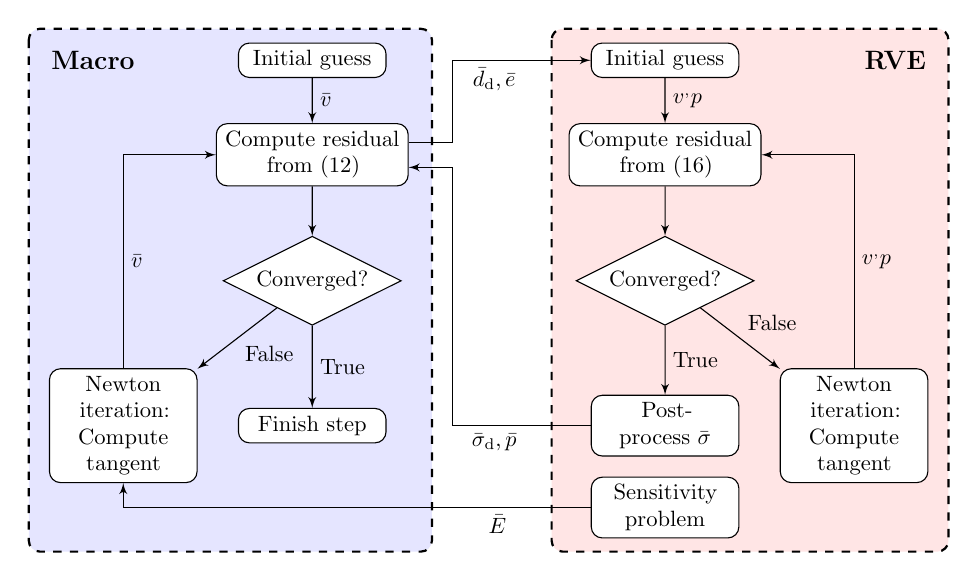
\begin{tikzpicture}[node distance = 2cm, auto,scale=0.8, transform shape, >=latex']
    %\small
    %\tikzstyle{every node}=[font=\footnotesize]
    \tikzstyle{group}    = [rectangle, draw, thick, dashed, text width=6em, text centered, rounded corners]
    \tikzstyle{decision} = [diamond,   draw, fill=white, aspect=2, node distance=2.5cm, inner sep=2pt]
    \tikzstyle{block}    = [rectangle, draw, fill=white, text width=6em, text centered, rounded corners]
    \tikzstyle{line}     = [draw, ->]

    \draw [thick, dashed, fill=blue!10, rounded corners] (-4.5,0.5) rectangle ( 1.9,-7.8);
    \draw [thick, dashed, fill=red!10,  rounded corners] ( 3.8,0.5) rectangle (10.1,-7.8);
    \node [below right, inner sep=10pt] at (-4.5,0.5) { \textbf{\large Macro} };
    \node [below left,  inner sep=10pt] at (10.1,0.5) { \textbf{\large RVE} };

    % Place nodes
    \node [block] (init) {Initial guess};
    \node [block, below of=init, text width=8em, node distance=1.5cm] (residual) {Compute residual from (12)};
    \node [decision, below of=residual,node distance=2cm] (convergence) {Converged?};
    \node [block, below of=convergence, node distance=2.3cm] (stop) {Finish step};
    \node [block, left of=stop, node distance=3cm] (update) {Newton iteration: Compute tangent};
    % Draw edges
    \path [line] (init) -- (residual) node[midway] {$\bar{\ta{v}}$};
    \path [line] (residual) -- (convergence);
    \path [line] (convergence) -- node {False} (update);
    \path [line] (convergence) -- node {True} (stop);
    \path [line] (update) |- node[near start,right] {$\bar{\ta{v}}$} (residual);

    % Place nodes
    \node [block, right of=init, node distance=5.6cm] (rve_init) {Initial guess};
    \node [block, below of=rve_init, text width=8em, node distance=1.5cm] (rve_residual) {Compute residual from (16)};
    \node [decision, below of=rve_residual, node distance=2cm] (rve_convergence) {Converged?};
    \node [block, below of=rve_convergence, node distance=2.3cm] (rve_stop) {Post-process $\bar{\ts\sigma}$};
    \node [block, right of=rve_stop, node distance=3cm] (rve_update) {Newton iteration: Compute tangent};
    % Sensitivity problem
    \node [block, below of=rve_stop, node distance=1.3cm] (rve_sensitivity) {Sensitivity problem};
    
    % Draw edges
    \path [line] (rve_init) -- (rve_residual) node[midway] {$\ta{v}^\fluct,p$};
    \path [line] (rve_residual) -- (rve_convergence);
    \path [line] (rve_convergence) -- node {False} (rve_update);
    \path [line] (rve_convergence) -- node {True} (rve_stop);
    \path [line] (rve_update) |- node[right, near start] {$\ta{v}^\fluct,p$} (rve_residual);

    \path [line] (residual.east) ++(0, 0.2cm) -- ++(0.7cm,0) |- node [below,pos=0.65] {$\bar{\ts d}_\dev, \bar{e}$} (rve_init);
    % Draw this backwards in order to get exact alignments
    \path [line, <-] (residual.east) ++(0,-0.2cm) -- ++(0.7cm,0) |- node [below,pos=0.65] {$\bar{\ts\sigma}_\dev, \bar{p}$} (rve_stop);

    \path [line] (rve_sensitivity) -| node[below, pos=0.10] {$\bar{\tf E}$} (update);
\end{tikzpicture}

% \end{center}
% \end{frame}

%%%%%%%%%%%%%%%%%%%%%%%%%%%%%%%%%%%%%%%%%%%%%%%%%%%%%%%%%%%%%%%%%%%%%%%%%%%%%%%%%%%%%%%%%%%%%%%%%%%
\begin{frame}
 \frametitle{Choice of prolongation}
\begin{itemize}
 \item First order Taylor expansion of the displacement, and zeroth order expansion of the pressure
\begin{align*}
 \ta u^\macro &= \bar{\ta u} + [\bar{\ta u}\outerp\diff]\cdot[\ta x - \bar{\ta x}]
\\
 p^\macro &= \bar{p}
\end{align*}
 \item Constraints on the fluctuations $\ta u^\fluct$ and $p^\fluct$ within each RVE via the conditions
\begin{align*}
 \homgen{\ta u\outerp\diff} &= \bar{\ta u}\outerp\diff
\\
 \homgen{p} &= \bar{p}
\end{align*}
\end{itemize}
\end{frame}

%%%%%%%%%%%%%%%%%%%%%%%%%%%%%%%%%%%%%%%%%%%%%%%%%%%%%%%%%%%%%%%%%%%%%%%%%%%%%%%%%%%%%%%%%%%%%%%%%%%
\begin{frame}
 \frametitle{Macroscale problem}
\begin{itemize}
 \item Find $(\bar{\ta u}, \bar{p}) \in \bar{\set U}\times \bar{\set P}$ such that
 \begin{align*}
  \int_\Omega [{\bar{\ts\sigma}_\dev\{\bar{\ts\epsilon}_\dev, \bar{p}\}} - \bar{p}\ts I]\dprod[\delta\bar{\ta u}\outerp\diff]\dif V &= 0\quad \forall \delta\bar{\ta u} \in \bar{\set{U}}^0
\\
  \int_\Omega [-\bar{\ta u}\cdot\diff + {\bar{e}\{\bar{\ts\epsilon}_\dev, \bar{p}\}}]\delta\bar{p}\dif V &= 0\quad \forall \delta\bar{p} \in \bar{\set{P}}
 \end{align*}
 \item RVE-input: $\bar{\ts\epsilon}_\dev\defeq [\bar{\ta u}\outerp\diff]^\sym_\dev$ and $\bar{p}$.
 \item Homogenized response variables identified as
 \begin{align*}
 \bar{\ts\sigma}_\dev &\defeq \frac{1}{\volume} \left[\int_{\Gamma_\rve} \ta t \outerp [\ta x-\bar{\ta x}]\dif S\right]_\dev
\\
 \bar{e} &\defeq \frac{1}{\volume} \int_{\Gamma_\rve} \ta u \cdot \ta n\dif S
 \end{align*}
\end{itemize}
\end{frame}

%%%%%%%%%%%%%%%%%%%%%%%%%%%%%%%%%%%%%%%%%%%%%%%%%%%%%%%%%%%%%%%%%%%%%%%%%%%%%%%%%%%%%%%%%%%%%%%%%%%
\begin{frame}
 \frametitle{RVE problem --- Weakly Periodic b.c.}
\begin{itemize}
 \item For given macroscale variables $\bar{\ts\epsilon}_\dev$ and $\bar{p}$, find ($\ta{u},p,\ta t, \bar{e})\in\set{U}_\rve\times\set{P}_\rve\times\set{T}_\rve\times\set R$ that solve the system
%----------------------------------------------------------------------------
\begin{flalign*}
  \downlight{\int_{\mathrlap{\Omega_\rve}} [\hat{\ts\sigma}_\dev([\ta u \outerp\diff]^\sym_\dev)-p\ts I]\dprod[\delta\ta u \outerp\diff] \dif V} - \int_{\mathrlap{\Gamma_\rve^+}} \ta t\cdot\jump{\delta\ta u}\dif S &\downlight{= 0}
\end{flalign*}
\vspace{-2em}
\begin{flalign*}
&&
  \downlight{\forall\;\delta\ta u \in \set U_\rve}
\\
  \downlight{\int_{\mathrlap{\Omega_\rve}} -\delta p[\ta u \cdot\diff - \hat{e}(p)] \dif V }&\downlight{= 0}
&
  \downlight{\forall\;\delta p \in \set P_\rve}
\\
  -\int_{\mathrlap{\Gamma_\rve^+}} \delta\ta t\cdot \jump{\ta u - \bar{e}\frac13\ta x} \dif S &= -\int_{\mathrlap{\Gamma_\rve^+}} \delta\ta t\cdot \jump{\highlight{\bar{\ts\epsilon}_\dev}\cdot\ta x} \dif S
&
  \forall\;\delta\ta t \in \set T_\rve
\\
  \int_{\mathrlap{\Gamma_\rve^+}} \ta t \cdot \jump{\frac13\ta x} \dif S \,\delta\bar{e} &= - \highlight{\bar{p}} \,\delta\bar{e}
&
  \forall\;\delta\bar{e} \in \set R
\end{flalign*}
 \item $\jump{\bullet} = $ difference of $\bullet$ between $\Gamma_\rve^+$ and $\Gamma_\rve^-$ (mirror point)
\end{itemize}
\end{frame}

%%%%%%%%%%%%%%%%%%%%%%%%%%%%%%%%%%%%%%%%%%%%%%%%%%%%%%%%%%%%%%%%%%%%%%%%%%%%%%%%%%%%%%%%%%%%%%%%%%%
\begin{frame}
 \frametitle{RVE problem --- Dirichlet and Neumann b.c.}
\begin{itemize}
 \item For given macroscale variables $\bar{\ts\epsilon}_\dev$ and $\bar{p}$ obtain $\bar{\ts\sigma}_\dev$ and $\bar{e}$:
 \begin{itemize}
  \item Dirichlet b.c.: find ($\ta{u},p,\bar{e})\in\set{U}'_\rve\times\set{P}_\rve\times\set R$
  \begin{itemize}
    \item Similar implementation to traditional Dirichlet b.c. only $\bar{e}$ is not controlled.
    \item $\bar{\ts\sigma}_\dev$ response is post-processed reaction forces on RVE-boundary.
  \end{itemize}
  \item Neumann b.c.: find ($\ta{u},p,\bar{\ts\sigma}_\dev)\in\set{U}_\rve\times\set{P}_\rve\times\set{R}^{3\times 3}_\dev$.
  \begin{itemize}
    \item Similar implementation to traditional Neumann b.c. only $\bar{p}$ is controlled.
    \item $\bar{e}$ response is post-processed from displacement on RVE-boundary.
  \end{itemize}
 \end{itemize}
\end{itemize}
\end{frame}

%%%%%%%%%%%%%%%%%%%%%%%%%%%%%%%%%%%%%%%%%%%%%%%%%%%%%%%%%%%%%%%%%%%%%%%%%%%%%%%%%%%%%%%%%%%%%%%%%%%
\begin{frame}
 \frametitle{FE\textsuperscript{2} summarized}
\begin{center}
 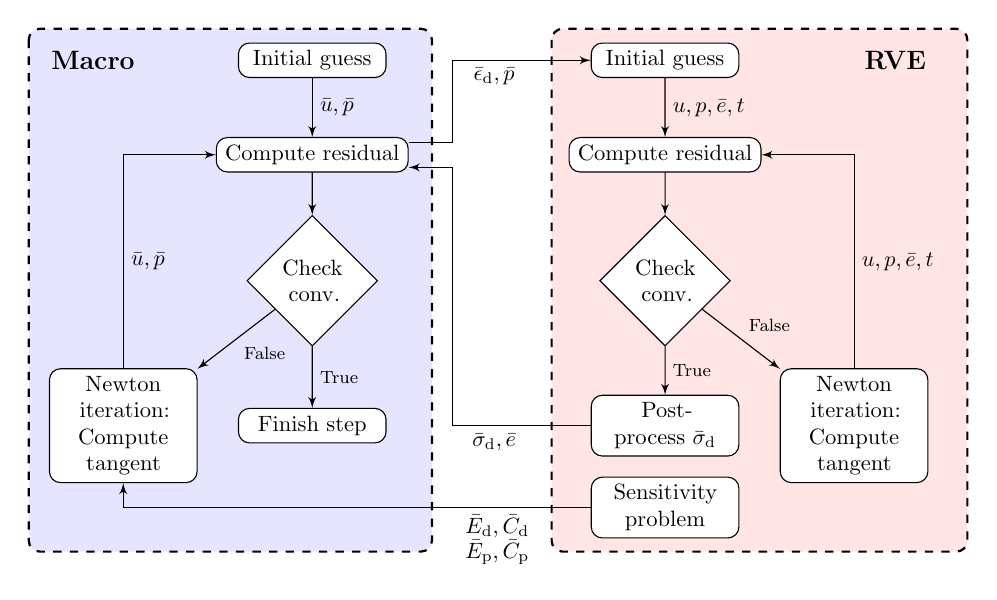
\begin{tikzpicture}[node distance = 2cm, auto,scale=0.8, transform shape]
    %\small
    %\tikzstyle{every node}=[font=\footnotesize]
    \tikzstyle{group}    = [rectangle, draw, thick, dashed, text width=6em, text centered, rounded corners]
    \tikzstyle{decision} = [diamond,   draw, fill=white, text width=4em, text centered, node distance=2.5cm, inner sep=0pt]
    \tikzstyle{block}    = [rectangle, draw, fill=white, text width=6em, text centered, rounded corners]
    \tikzstyle{line}     = [draw, -latex']

    \draw [thick, dashed, fill=blue!10, rounded corners] (-4.5,0.5) rectangle ( 1.9,-7.8);
    \draw [thick, dashed, fill=red!10,  rounded corners] ( 3.8,0.5) rectangle (10.4,-7.8);
    \node [below right, inner sep=10pt] at (-4.5,0.5) { \textbf{\large Macro} };
    \node [below left,  inner sep=10pt] at (10.1,0.5) { \textbf{\large RVE} };

    % Place nodes
    \node [block] (init) {Initial guess};
    \node [block, below of=init, text width=8em, node distance=1.5cm] (residual) {Compute residual};
    \node [decision, below of=residual,node distance=2cm] (convergence) {Check conv.};
    \node [block, below of=convergence, node distance=2.3cm] (stop) {Finish step};
    \node [block, left of=stop, node distance=3cm] (update) {Newton iteration: Compute tangent};
    % Draw edges
    \path [line] (init) -- (residual) node[midway] {$\bar{\ta{u}},\bar{p}$};
    \path [line] (residual) -- (convergence);
    \path [line] (convergence) -- node {\footnotesize False} (update);
    \path [line] (convergence) -- node {\footnotesize True} (stop);
    \path [line] (update) |- node[near start,right] {$\bar{\ta{u}},\bar{p}$} (residual);

    % Place nodes
    \node [block, right of=init, node distance=5.6cm] (rve_init) {Initial guess};
    \node [block, below of=rve_init, text width=8em, node distance=1.5cm] (rve_residual) {Compute residual};
    \node [decision, below of=rve_residual, node distance=2cm] (rve_convergence) {Check conv.};
    \node [block, below of=rve_convergence, node distance=2.3cm] (rve_stop) {Post-process $\bar{\ts\sigma}_\dev$};
    \node [block, right of=rve_stop, node distance=3cm] (rve_update) {Newton iteration: Compute tangent};
    % Sensitivity problem
    \node [block, below of=rve_stop, node distance=1.3cm] (rve_sensitivity) {Sensitivity problem};
    
    % Draw edges
    \path [line] (rve_init) -- (rve_residual) node[midway] {$\ta{u},p,\bar{e},\ta{t}$};
    \path [line] (rve_residual) -- (rve_convergence);
    \path [line] (rve_convergence) -- node {\footnotesize False} (rve_update);
    \path [line] (rve_convergence) -- node {\footnotesize True} (rve_stop);
    \path [line] (rve_update) |- node[right, near start] {$\ta{u},p,\bar{e},\ta{t}$} (rve_residual);

    \path [line] (residual.east) ++(0, 0.2cm) -- ++(0.7cm,0) |- node [below,pos=0.65] {$\bar{\ts \epsilon}_\dev, \bar{p}$} (rve_init);
    % Draw this backwards in order to get exact alignments
    \path [line, latex'-] (residual.east) ++(0,-0.2cm) -- ++(0.7cm,0) |- node [below,pos=0.65] {$\bar{\ts\sigma}_\dev, \bar{e}$} (rve_stop);

    \path [line] (rve_sensitivity) -| node[below, pos=0.10] {$\substack{\displaystyle\bar{\tf E}_\ded,\bar{\ts C}_\ded \\ \displaystyle\bar{\ts E}_\dep,\bar{C}_\dep}$} (update);
\end{tikzpicture}

\end{center}
\end{frame}

%%%%%%%%%%%%%%%%%%%%%%%%%%%%%%%%%%%%%%%%%%%%%%%%%%%%%%%%%%%%%%%%%%%%%%%%%%%%%%%%%%%%%%%%%%%%%%%%%%%
\begin{frame}
 \frametitle{Statistical Volume Element (SVE)}
\begin{center}
 \hspace{1cm}
 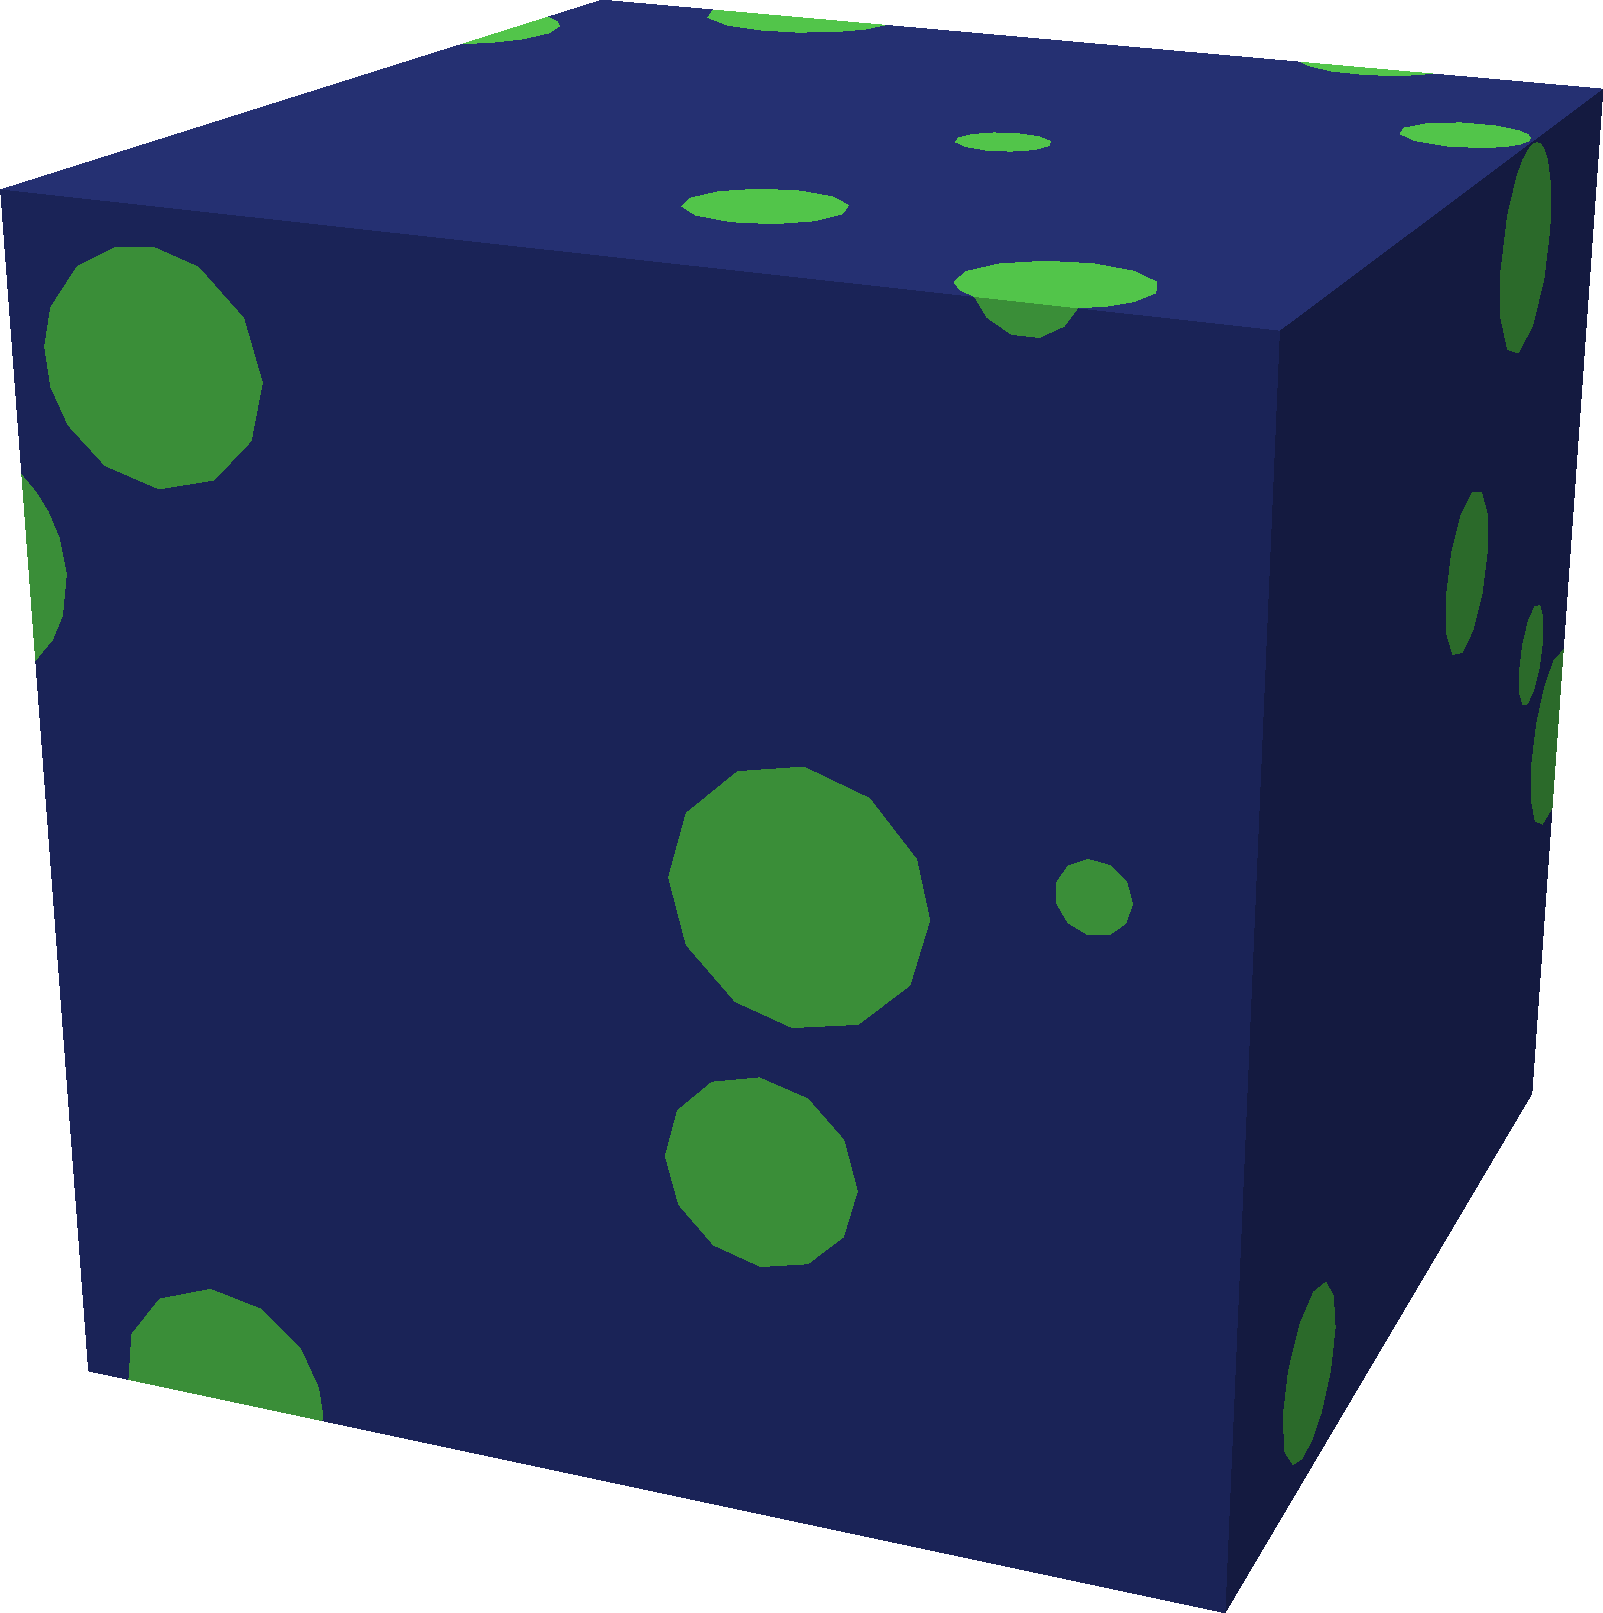
\includegraphics[scale=0.05]{figures/rve6.png}
 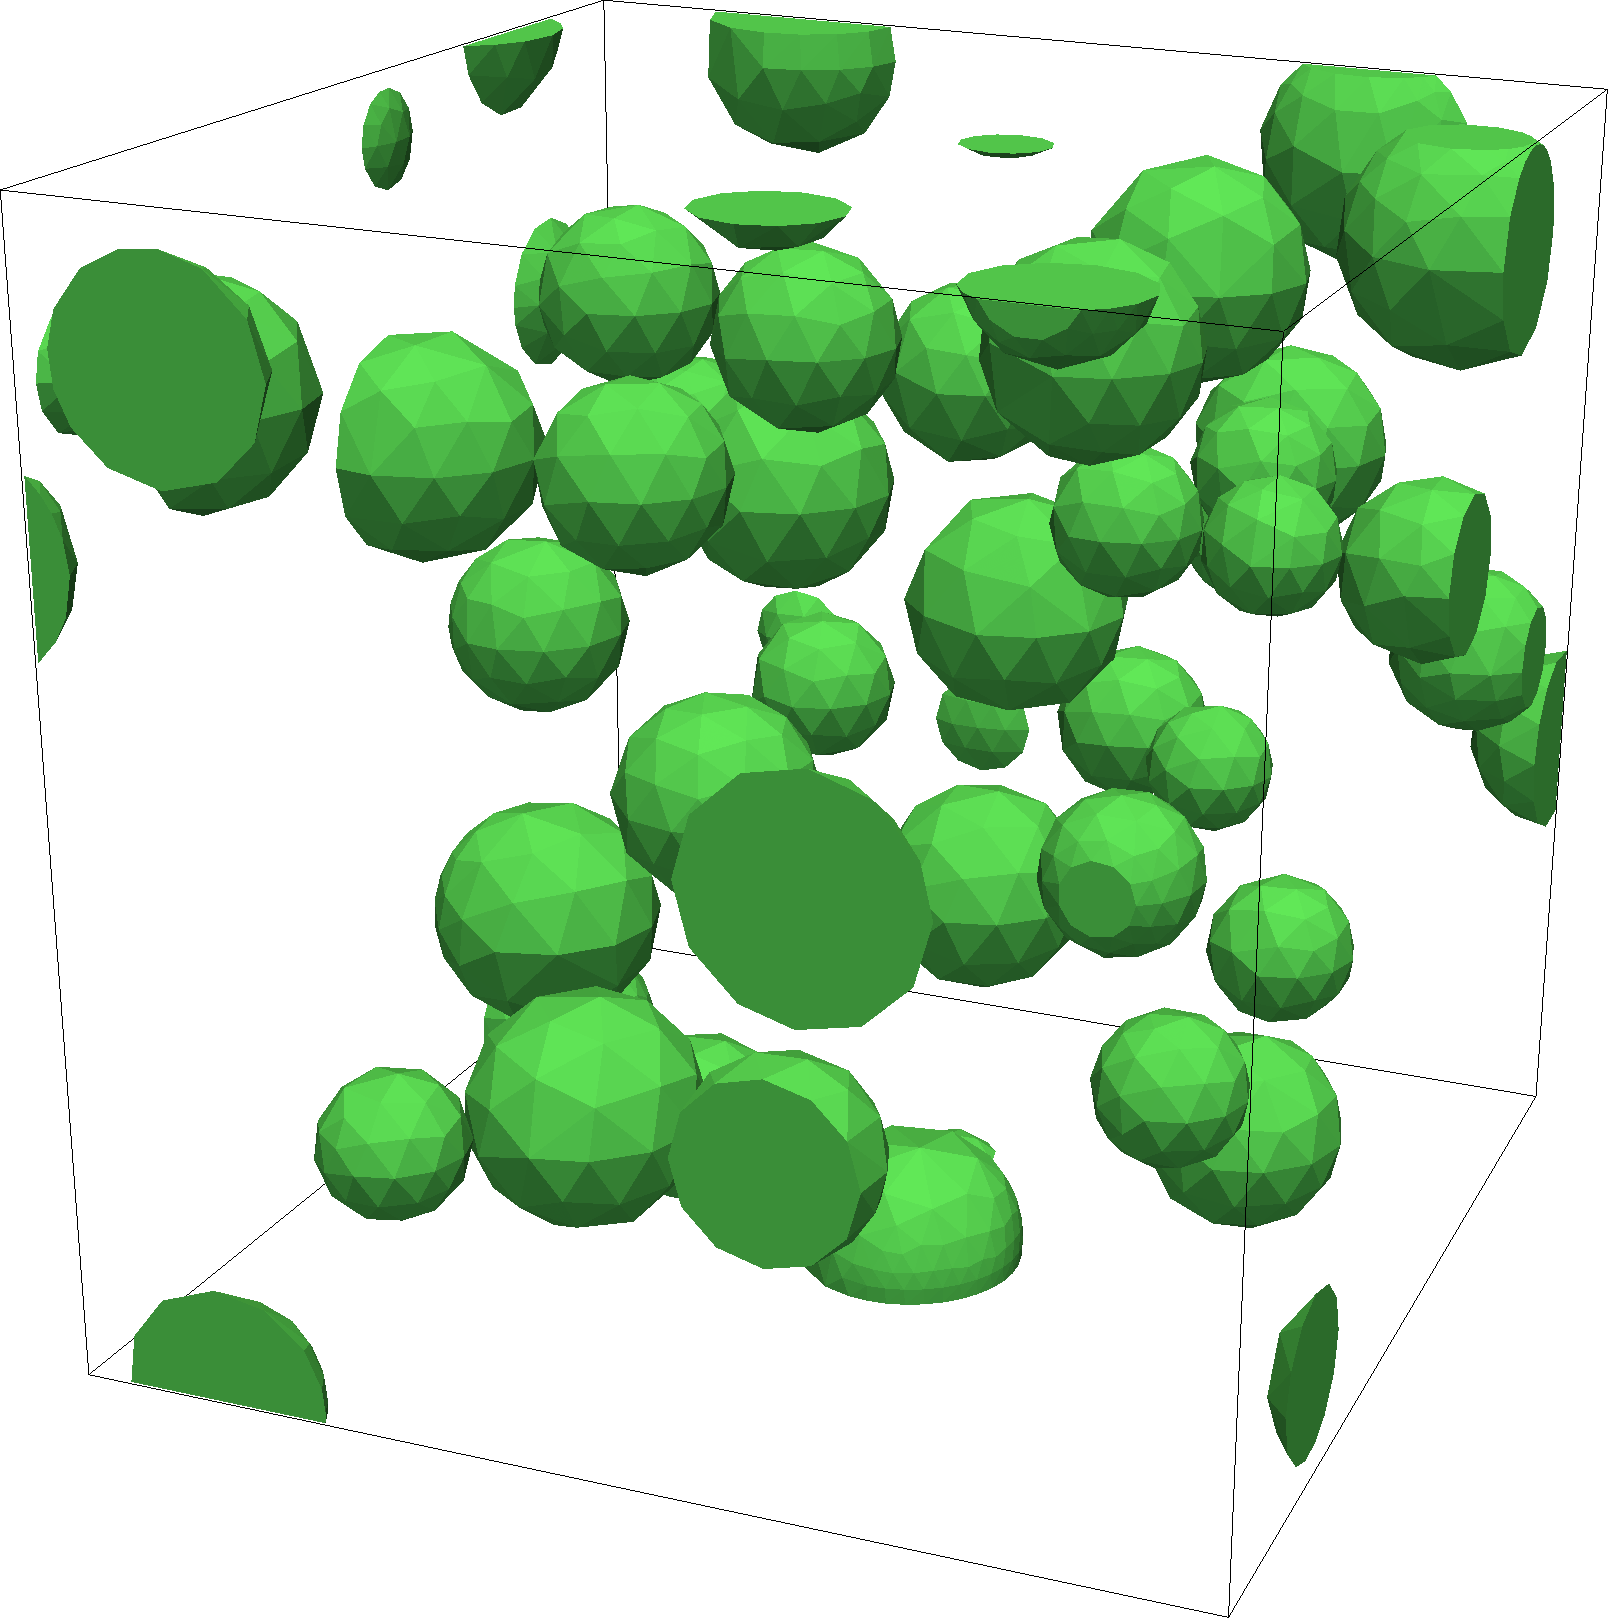
\includegraphics[scale=0.05]{figures/rve6_inc.png}
 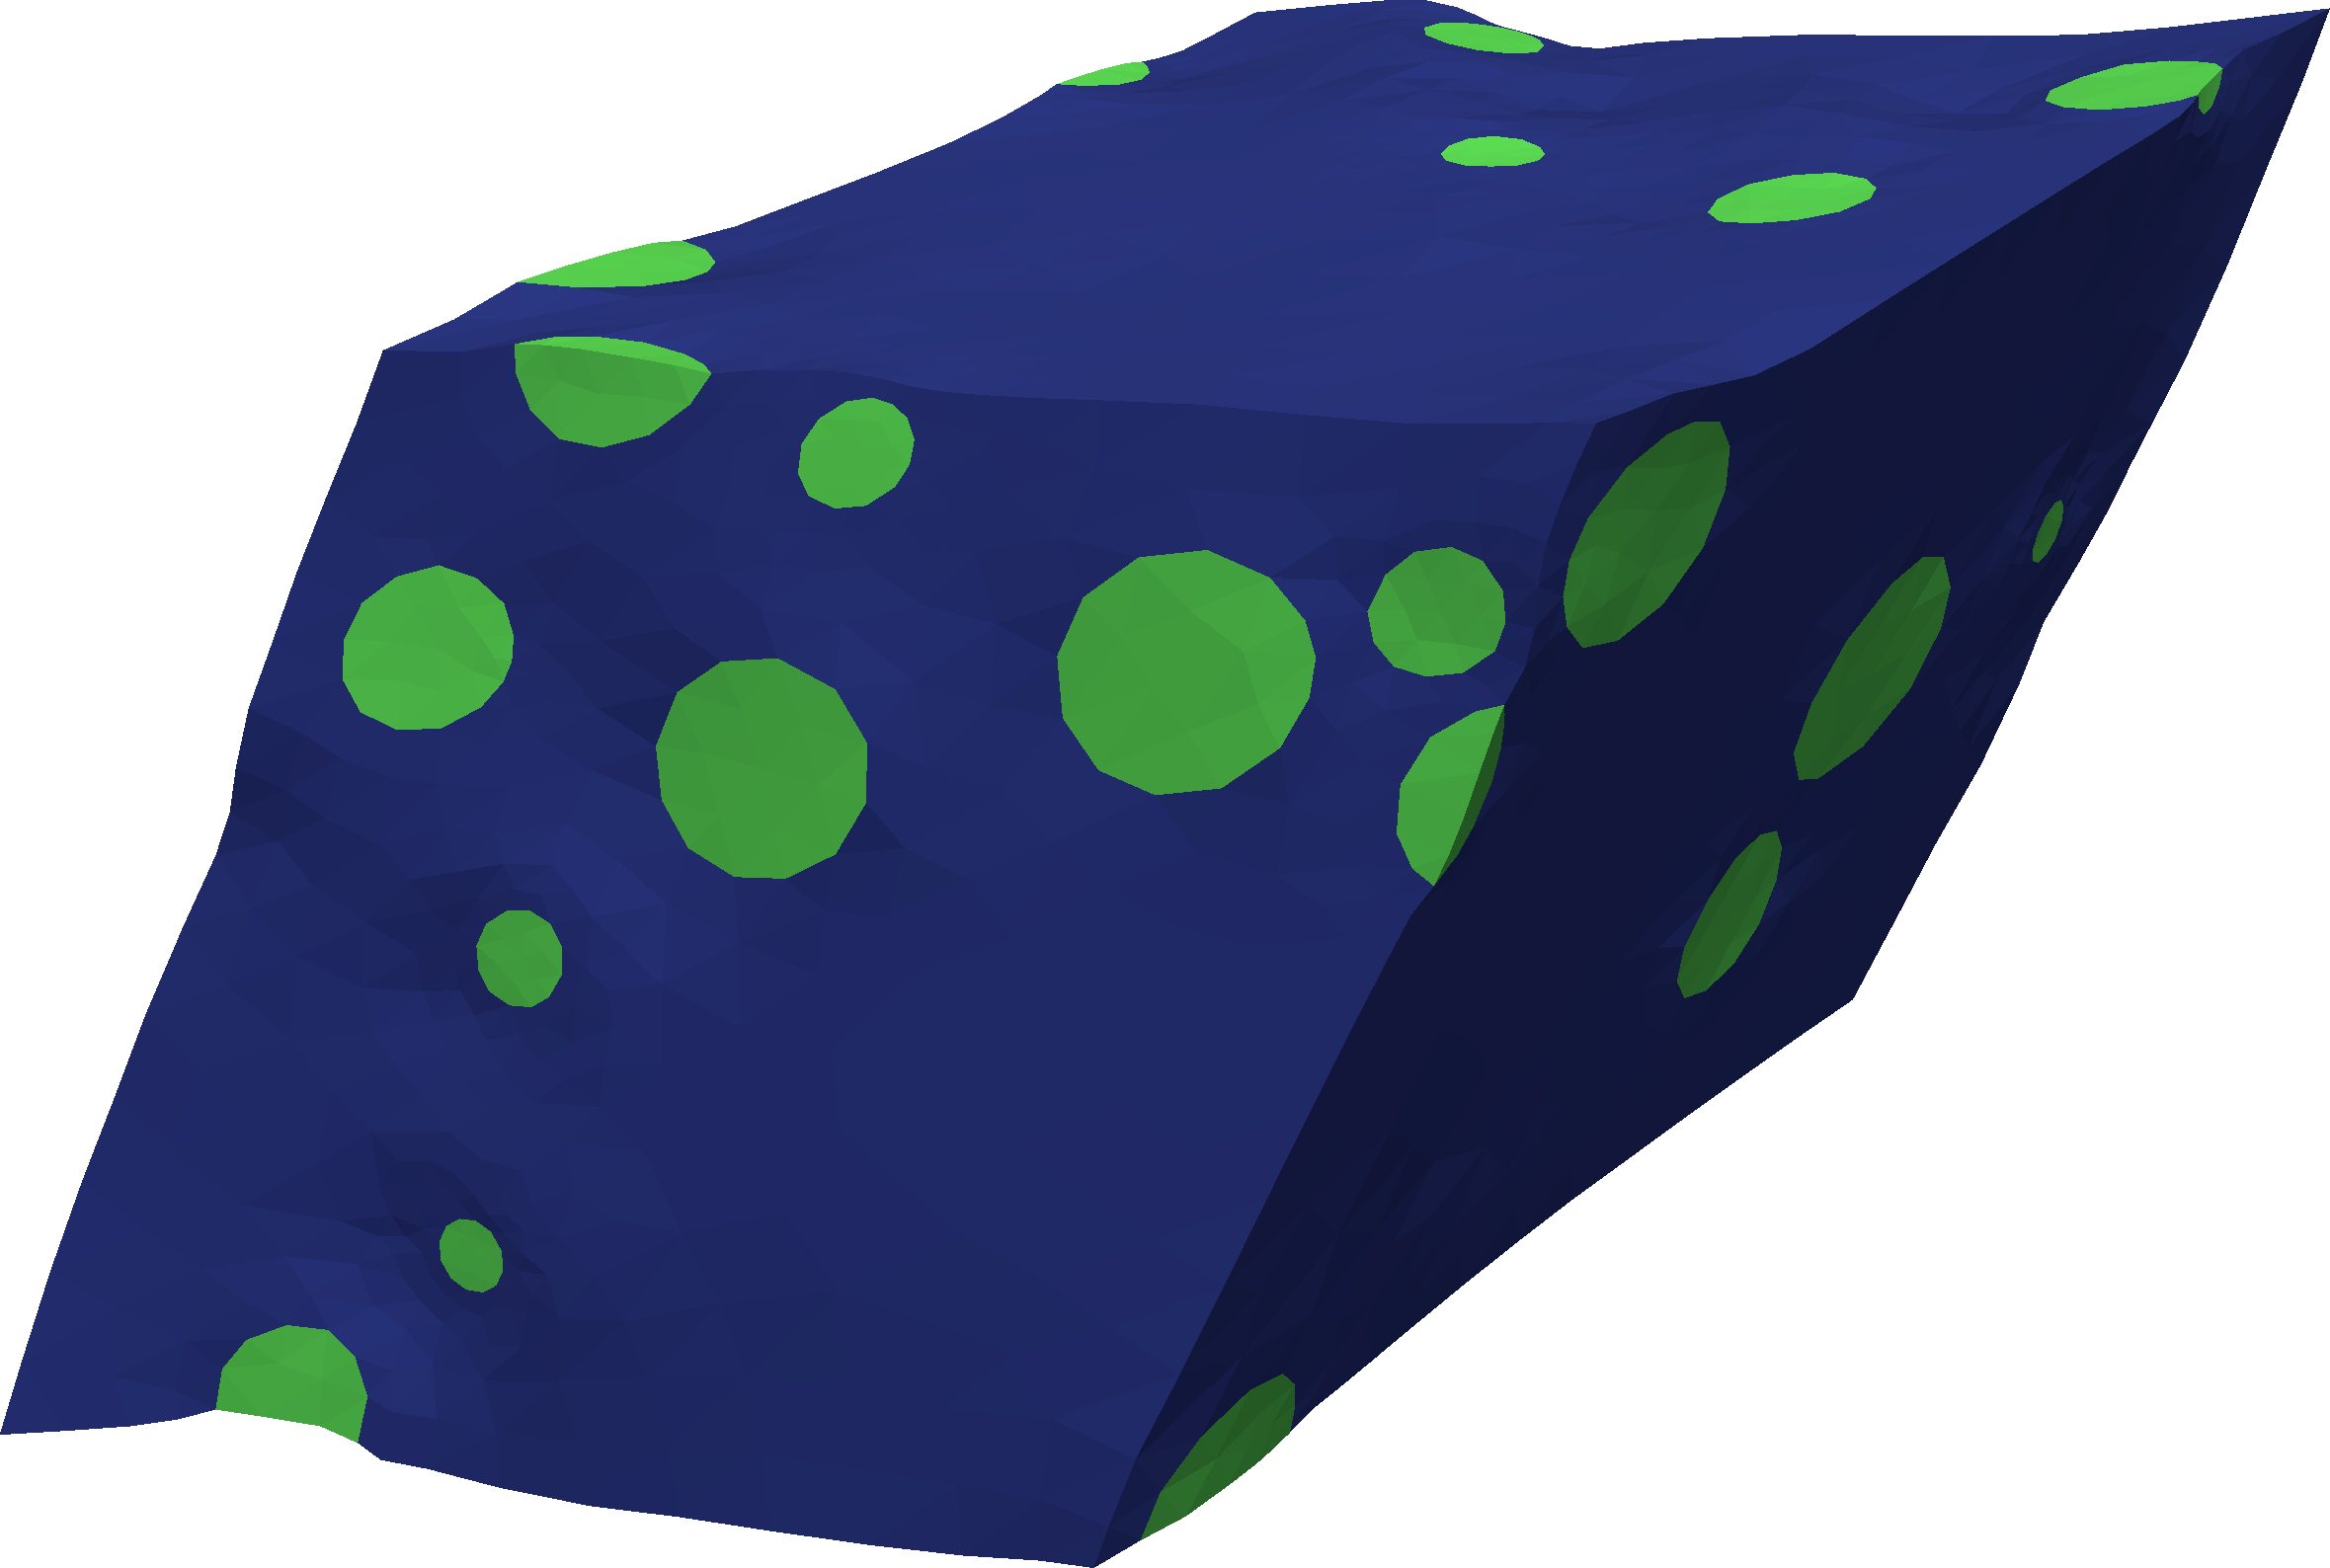
\includegraphics[scale=0.05]{figures/rve6_def.png}
\end{center}
 \begin{align*}
  \hat{\ts\sigma}_\dev(\ts\epsilon_\dev) &= 2 G \ts\epsilon_\dev
\\
  \hat{e}(p) &= -C p = -\frac{1}{K} p
 \end{align*}
\end{frame}

%%%%%%%%%%%%%%%%%%%%%%%%%%%%%%%%%%%%%%%%%%%%%%%%%%%%%%%%%%%%%%%%%%%%%%%%%%%%%%%%%%%%%%%%%%%%%%%%%%%
\begin{frame}
 \frametitle{Homogenized shear and bulk modulus}
\begin{center}
%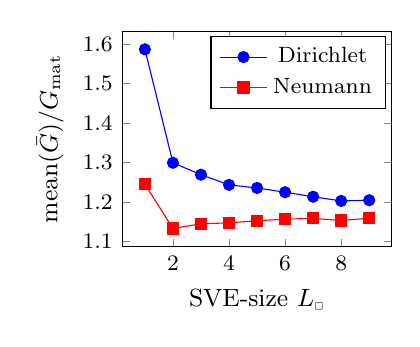
\begin{tikzpicture}
  \begin{axis}[ width=0.5\linewidth, height=0.28\linewidth,
      footnotesize,
      xlabel=SVE-size $L_\rve$, ylabel=$\mathop{\mathrm{mean}}(\bar{G})/G_\mathrm{mat}$]
  \addplot table[color=blue,x=size,y=d_mean] {
size d_mean d_var
1.000000   1.586624   0.489829
2.000000   1.299371   0.029517
3.000000   1.269267   0.007279
4.000000   1.243507   0.002562
5.000000   1.235669   0.000874
6.000000   1.224925   0.000534
7.000000   1.213449   0.000258
8.000000   1.202848   0.000205
9.000000   1.204560   0.000033
  };
 \addlegendentry{Dirichlet}
  \addplot table[color=red,x=size,y=n_mean] {
size n_mean n_var
1.000000   1.245017   0.110729
2.000000   1.133016   0.006438
3.000000   1.144928   0.002252
4.000000   1.147371   0.001132
5.000000   1.152570   0.000572
6.000000   1.156771   0.000293
7.000000   1.158645   0.000139
8.000000   1.153319   0.000129
9.000000   1.158993   0.000039
  };
\addlegendentry{Neumann}
  \end{axis}
\end{tikzpicture}

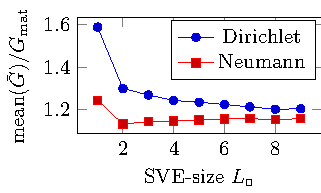
\includegraphics[width=0.4\linewidth]{figures/meanG}
%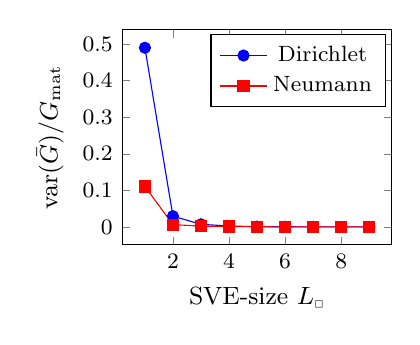
\begin{tikzpicture}
  \begin{axis}[ width=0.50\linewidth, height=0.28\linewidth,
      footnotesize,
      xlabel=SVE-size $L_\rve$, ylabel=$\mathop{\mathrm{var}}(\bar{G})/G_\mathrm{mat}$]
  \addplot table[color=blue,x=size,y=d_var] {
size d_mean d_var
1.000000   1.586624   0.489829
2.000000   1.299371   0.029517
3.000000   1.269267   0.007279
4.000000   1.243507   0.002562
5.000000   1.235669   0.000874
6.000000   1.224925   0.000534
7.000000   1.213449   0.000258
8.000000   1.202848   0.000205
9.000000   1.204560   0.000033
  };
\addlegendentry{Dirichlet}
  \addplot table[color=red,x=size,y=n_var] {
size n_mean n_var
1.000000   1.245017   0.110729
2.000000   1.133016   0.006438
3.000000   1.144928   0.002252
4.000000   1.147371   0.001132
5.000000   1.152570   0.000572
6.000000   1.156771   0.000293
7.000000   1.158645   0.000139
8.000000   1.153319   0.000129
9.000000   1.158993   0.000039
  };
\addlegendentry{Neumann}
  \end{axis}
\end{tikzpicture}

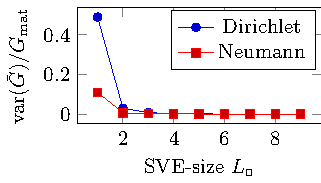
\includegraphics[width=0.4\linewidth]{figures/varG}
\\
$G_\mathrm{part} = 5 G_\mathrm{mat}$, $C_\mathrm{part} = C_\mathrm{mat} = 0$
\\%hline
%\begin{tikzpicture}
  \begin{axis}[ 
    width=0.45\linewidth, height=0.28\linewidth,
    xlabel=$C_\mathrm{mat}\times G_\mathrm{mat}$,
    ylabel=$\bar{C}\times G_\mathrm{mat}$,
    extra x ticks={1.09091, 0.75000, 0.46154, 0.21429, 0.00000},
    extra x tick labels={0.1, 0.2, 0.3, 0.4, 0.5}, 
    every extra x tick/.style = {
        xticklabel style = {name=name label},
        xtick pos = right,
        xticklabel pos = right,
        xtick align = outside
    }
    ]
  \addplot table[color=blue,x=M,y=C] {macro_k9.matdata};
  \end{axis}
  \node at (2.1,2.8) { $\nu_\mathrm{mat}$ };
\end{tikzpicture}

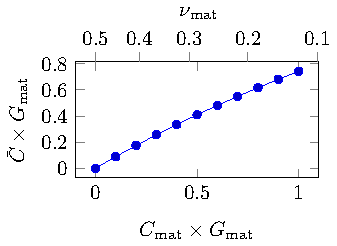
\includegraphics[width=0.4\linewidth]{figures/CGmat}
%\begin{tikzpicture}
  \begin{axis}[
    width=0.45\linewidth, height=0.28\linewidth,
    xlabel=$C_\mathrm{mat}\times G_\mathrm{mat}$,
    ylabel=$\bar{G}/G_\mathrm{mat}$,
    extra x ticks={1.09091, 0.75000, 0.46154, 0.21429, 0.00000},
    extra x tick labels={0.1, 0.2, 0.3, 0.4, 0.5}, 
    every extra x tick/.style = {
        xticklabel style = {name=name label},
        xtick pos = right,
        xticklabel pos = right,
        xtick align = outside
    }
    ]
  \addplot table[color=blue,x=M,y=G] {macro_k9.matdata};
  \end{axis}
  \node at (2.1,2.8) { $\nu_\mathrm{mat}$ };
\end{tikzpicture}

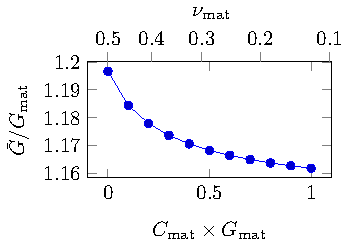
\includegraphics[width=0.4\linewidth]{figures/GGmat}
\\
$G_\mathrm{part} = 5 G_\mathrm{mat}$, $C_\mathrm{part} = 0$
% Homogenized results from a single RVE with Dirichlet boundary condition.
% Dependence of effective properties $\bar{C}$ and $\bar{G}$ on the bulk compliance $C_\mathrm{mat}$ for fixed values of $G_\mathrm{part} = 5\,G_\mathrm{mat}$ and $C_\mathrm{part} = 0$.
\end{center}
\end{frame}

%%%%%%%%%%%%%%%%%%%%%%%%%%%%%%%%%%%%%%%%%%%%%%%%%%%%%%%%%%%%%%%%%%%%%%%%%%%%%%%%%%%%%%%%%%%%%%%%%%%
\begin{frame}
 \frametitle{Conclusions}
 \begin{itemize}
 \item Seamless transition to macroscopic incompressibility
 \item Methodology is extensible to include pores and surface tension
 %\item Modified Neumann-b.c. at no additional computational cost
 \item Implementation available in the open source code OOFEM \texttt{www.oofem.org}
 \end{itemize}
\end{frame}

\end{document}
